%!TEX TS-program = xelatex
%!TEX encoding = UTF-8 Unicode

\documentclass{../../lib/gs}

% Configurazione per URL su nuova linea
\DeclareFieldFormat{url}{\newline\footnotesize\url{#1}}
\DeclareFieldFormat{howpublished}{\newline\footnotesize#1}
\DeclareFieldFormat{urldate}{\mkbibparens{#1}}

\usepackage{../../lib/apf}

% Packages per figure e grafici
\usepackage{pgfplots}
\pgfplotsset{compat=1.18}
\usepackage{tikz}
\usetikzlibrary{decorations.text}
\usepackage{subcaption}

\usepackage{enumitem}

\title{il sogno radicale}
\subtitle{autobiografia di un eretico. appunti revb.}
\author{Giuseppe Silvi}
\date{\today}

% Definizione delle parole chiave per i metadati PDF
\kuno{filosofia}
\kdue{greco antico}
\ktre{Platone}
\kquattro{etimologia}
\kcinque{XeLaTeX}

% Comandi per la notazione AllPass
\newcommand{\apf}[3]{\textbf{\texttt{#1(#2,#3)}}}
\newcommand{\apfc}[3]{\begin{center}\apf{#1}{#2}{#3}\end{center}}
\newcommand{\apfcn}[4]{\begin{center}\apf{#1}{#2}{#3}\footnote{#4}\end{center}}

% Nel preambolo del .tex
\addbibresource{../bibliografia.bib}

\begin{document}

\maketitle

\addcontentsline{toc}{section}{premessa: \emph{perché siamo qui?}}
\section*{premessa: \emph{perché siamo qui?}}

Sto operando quella che Ronchi, nella prefazione de \emph{Il pensiero bastardo}
\cite{ronchi2001} ha definito una «torsione», una «preliminare torsione
filosofica» dell'oggetto.

\begin{quote}
\begin{sf}
\small
  Le altre pratiche (pittura, fotografia, cinema, ecc.) sono chiamate in causa
  solo al prezzo di una preliminare torsione filosofica del loro oggetto.
  \cite{ronchi2001}
  \end{sf}
\end{quote}

\textit{Torsiō} deriva dal verbo \textit{torquēre}, riconducibile alla radice
indoeuropea *terkʷ- “torcere, girare”\footnote{Pokorny IEW 1077-1078; de Vaan
EDLIL 621-622.}, che designa il movimento rotatorio applicato mediante forza.
La torsione implica una resistenza\footnote{Il materiale oppone una resistenza
caratterizzata dal modulo di elasticità tangenziale e dal momento d'inerzia
polare della sezione. Dal latino \emph{re-sistere}: uno \emph{stare contro} che
è inevitabilmente anche \emph{stare di nuovo} - un ristabilirsi, un tornare a
stare.} che rende possibile una tensione\footnote{La torsione genera tensioni di
taglio (\emph{shear stress}) nel materiale. Queste tensioni sono distribuite
trasversalmente alla sezione e aumentano linearmente dalla fibra neutra verso
la periferia. Dal latino \emph{tensio}, da \emph{tendere}, pro-tendere qualcosa
verso; un orientamento attivo.}. Un \emph{ob-ponere} istantaneo che dura in un
\emph{ob-sidere}, quindi in una forma, in un movimento. Un doppio moto – di
deformazione sotto l'azione del momento torcente applicato; di ritorno ad un
altro momento sotto l'azione di resistenza elastica\footnote{Il termine momento
indica sia l'istante temporale che la grandezza fisica (momento torcente),
suggerendo come ogni deformazione sia sempre un dialogo tra forza e tempo, tra
imposizione e memoria del materiale. Ritorno ad un altro momento perché, dopo
una torsione, si è altrove.}.

\begin{figure}[htbp]
\begin{center}
\begin{tikzpicture}
  \tikzstyle{every node}=[font=\small]
  \ciclodiagram{torsione}{resistenza}{tensione}
\end{tikzpicture}
\caption{Il grafico simboleggia la torsione come nodo concettuale stretto tra un
moto di tensione distorcente e un moto di ritorno sotto la forza di resistenza.}
\label{torsione}
\end{center}
\end{figure}

Mi è evidente che c'è un passo della torsione, quello successivo, che conduce
alla \emph{dis}-torsione. Tuttavia, seppur con questo breve pensiero cerco di
tenermene a distanza, un passo prima, mi è altresì evidente che, in torsione,
non si può avere paura delle distorsioni poiché questa impedirebbe possibili
\emph{con}-torsioni. È se anche il Prof. Ronchi intendesse indicare una qualsiasi
semplice deviazione rispetto a una condizione di normalità o linearità (la
torsione di un ragionamento, di una interpretazione, di una situazione), cosa
che io dubito, ormai mi son mosso.

Sento un'assenza. Mi accorgo, quotidianamente, da un certo tempo, a seguito di
alcune singole riflessioni \cite{silvi2023a, silvi2023b, silvi2023c, silvi2024},
seppur non isolate, di desiderare, di avere necessità di \emph{abitare} una
teoria della musica. Non è un bisogno, momentaneo e transitorio, bensì
l'inevitabile presenza di un'assenza, costante. Molte delle singole riflessioni,
delle risonanze singolari, vorrebbero appartenere a un riverbero, a riverberi
generali di un luogo più ampio che chiamerei \emph{teoria della musica}.

\begin{quote}
\begin{sf}
\small
  La teoria è infatti chiamata in causa, dopotutto, solo per far luce su di
  un'esperienza di cui non si riesce a venire a capo. \cite{ronchi2001}
  \end{sf}
\end{quote}

Abitare una teoria. Tuttavia, \emph{che cos'è una teoria? Che cos'è una teoria
musicale? E santo cielo! Che cos'è Musica? E poi che cos'è un'esperienza? Che
cos'è un'esperienza musicale?}

Heidegger, che mi pare amasse le torsioni, in un ragionamento sull'abitare
\cite{heidegger1991} si muove da un primo passo «All'abitare, così sembra,
perveniamo solo attraverso il costruire». Questo mi fa pensare che noi oggi, in
musica, siamo in piena «crisi di alloggi». Osservo l'ambiente che mi circonda e
vedo pochissime costruzioni che «albergano l'uomo», il musicista. edifici vecchi,
consumati o restaurati per le nuove forme di turismo (musicale). Per imparare
ad avere rispetto della mia ineluttabile necessità scorro la storia delle teorie
della musica, un indice che si muove più volte avanti e dietro, non in cerca di
regole, definizioni di una o più problematiche specifiche, ma in cerca di
divergenze, di attitudini, di problematiche generali affinché io possa, con
semplicità, trovare radici per le mie problematiche specifiche, per le utopie
che muovono le mani. «Il costruire non è soltanto mezzo e via per l'abitare, il
costruire è già in se stesso un abitare.» \cite{heidegger1991}

\begin{quote}
\begin{sf}
\small
  L'incontro fra due discipline non avviene quando l'una si mette a riflettere sull'altra, ma quando una si accorge di dover risolvere per conto proprio e
  con i propri mezzi un problema simile a quello che si pone anche in un'altra.
  [\ldots] Sono le medesime scosse in terreni completamente diversi.
  [\ldots] Non c'è opera che non abbia il suo seguito o il suo inizio in altre
  arti.
  \cite{deleuze2009}
  \end{sf}
\end{quote}

% \vspace{1cm}
%
% NOTA: mettere in relazione il costruire con «il loro oggetto” di Ronchi.

\clearpage

\section{\emph{en archei}}

\begin{quote}
\begin{sf}
\small
Dove ha origine – ci si chiede in queste pagine – il fascino che accompagna l'apparizione di qualcosa quando questo si staglia dal suo contesto abituale per lasciare traccia del suo passaggio?
\end{sf}
\end{quote}

\emph{dove ha origine?}

È un dove nasce e, insieme, un quando inizia. Ma è anche un quando nasce e, insieme, un dove inizia. \emph{Origins}, punto di partenza temporale oriente, \emph{oriens}, che sorge. Dove ha origine è una corrispondenza spazio–temporale. Un \emph{archē}.


\begin{quote}
\begin{sf}
\small
L'archeologia è la ricerca di un \emph{archē}, ma il termine greco \emph{archē} ha due significati: significa tanto “origine, principio”, quanto “comando ordine”. Così, il verbo \emph{archo} significa “iniziare, essere il primo a fare qualcosa” ma significa anche “comandare, essere il capo”. Senza dimensione che l'arconte (letteralmente “colui che comincia”) era in Atene la suprema magistratura. \cite{agamben2017}
\end{sf}
\end{quote}

\emph{En archei}, in principio, nel comando, «cioè nella forma di un comando», «l'inizio è sempre anche il principio che governa e comanda».

Archeologia del fascino che accompagna l'apparizione. Qualcosa appare e nell'apparire ammalia. Qualcosa appare e nell'apparire si lega insieme all'apparizione, come una fase che vincola e attrae irresistibilmente. L'archeologia del fascino mantiene l'idea di un potere che opera al di là della volontà razionale, \emph{en archei}, il potere di un comando. «Qualcosa appare a partire da se stesso» \cite{agamben2019} Apparire, mostrarsi, divenire visibile a partire da se stesso. È un \emph{ad – parēre}, un movimento verso.

\begin{quote}
\begin{sf}
\small
Il presente, l'\emph{Anwesend}, deve avermi già rivolto la parola nel suo essere presente. \cite{agamben2019}
\end{sf}
\end{quote}

C'è un qualcosa. C'è un movimento. C'è un qualcosa che si muove. C'è un fascino che accompagna il qualcosa in movimento. Ha tutti i tratti per essere definito un segnale: mezzo – movimento – informazione\footnote{attenzione: Ronchi dedica il libro al passaggio della cometa halle Bopp. APPROFONDIRE}.

\begin{quote}
\begin{sf}
\small
  Ciò che è al presente è quello che l'immagine “rappresenta”, ma non l'immagine
  stessa. L'immagine è un insieme di rapporti di tempo, da cui scaturisce il
  presente come comune multiplo o come minimo divisore. I rapporti di tmepo non
  sono mai visibili nella percezione ordinaria, ma lo sono nell'immagine, non
  appena essa diventa creatrice. L'immagine rende sensibili, visibili, i rapporti
  di tmepo irriducibli al presente.
  \cite{deleuze2009}
  \end{sf}
\end{quote}

\begin{quote}
\begin{sf}
\small
  Non c'è un inizio così come non c'è una fine. Si arriva sempre nel mezzo di
  qualcosa, si crea solo nel mezzo, dando nuove direzioni o biforcazini a delle
  linee che preesistono.
  \cite{deleuze2009}
  \end{sf}
\end{quote}

%-------------------------------------------------------------------------------
%----------------------------------------------------------------- SUB-SECTION -
%-------------------------------------------------------------------------------

\subsection{\emph{ichnos}}

Il termine \textit{ichnos} (ἴχνος) affonda le sue radici nella proto-lingua indoeuropea attraverso la radice \textit{*seik-} o \textit{*seig-}, che veicola l'idea fondamentale di "raggiungere", "estendersi" o "toccare" \cite{chantraine1968}. Questa radice si ritrova in diverse lingue della famiglia indoeuropea: nel sanscrito \textit{siṣakti} (egli cerca), nel germanico antico \textit{*saikjan-} (cercare), nel latino \textit{signum} (segno, marca).

La peculiarità del greco \textit{ichnos} risiede nella specificazione semantica verso il concetto di “impronta del piede”, ma con un'estensione metaforica verso qualsiasi tipo di traccia o segno lasciato da un passaggio. Il verbo correlato \textit{ἰχνεύω} (ichneuo) significa “seguire le tracce”, “investigare”, “rintracciare”, introducendo una dimensione dinamica e processuale.

Nei testi omerici, \textit{ichnos} compare principalmente in contesti venatori o militari, designando le tracce che permettono di seguire una preda o un nemico. Tuttavia, già in Pindaro troviamo un uso metaforico del termine per indicare la “via” o il “percorso” \cite{pindar1997}.

Nei frammenti di Parmenide, l'idea di traccia si lega alla questione dell'essere e del non-essere, mentre in Platone la nozione di \textit{typos} (τύπος) - intimamente connessa a \textit{ichnos} - diventa centrale nella teoria delle idee come "impronte" impresse sulla materia.

Il termine “traccia”, dal latino medievale \textit{tractiare} (frequentativo di \textit{trahere}), introduce una dimensione temporale specifica: quella della successione e della direzione. A differenza dell'\textit{ichnos} greco, che può indicare anche un segno statico, “traccia” implica sempre movimento e processualità, il segno di un passaggio che orienta verso una direzione futura.

%La traccia non è mai un semplice residuo passivo, ma il segno di un passaggio che orienta verso una direzione futura. In Levinas, la traccia dell'Altro è precisamente ciò che eccede ogni presente, ogni presenza possibile, orientando verso un'alterità irriducibile \cite{levinas1974}.

“Impronta”, da \textit{imprimere} (premere sopra), evoca la dinamica del contatto diretto, della forza che si esercita su una superficie. Questo termine porta con sé una dimensione di necessità fisica che manca negli altri due: l'impronta testimonia un incontro reale, una resistenza vinta, una forma imposta. L'impronta è sempre il risultato di una relazione, di un contatto che trasforma simultaneamente il soggetto imprimente e l'oggetto che riceve l'impressione \cite{merleau-ponty1945}.

“Vestigio”, dal latino \textit{vestigium}, introduce la dimensione della perdita e della frammentarietà. Il vestigio è ciò che resta \textit{in quanto} resto, ciò che porta in sé il segno della propria incompletezza essenziale, è forma specifica di apparizione del tempo storico. Il vestigio rende visibile la dialettica tra natura e storia, mostrando come ogni costruzione culturale porti in sé i semi della propria dissoluzione \cite{benjamin1928}.

%\subsection{Archeologia della coscienza temporale}

L'analisi husserliana della coscienza interna del tempo \cite{husserl1928} offre uno strumento concettuale per comprendere come la triplice articolazione traccia-impronta-vestigio operi nella costituzione dell'esperienza temporale soggettiva.

La \textit{ritenzione} primaria corrisponde alla modalità della traccia: è il processo attraverso cui il presente appena trascorso viene "trattenuto" nella coscienza, creando quella continuità temporale che Husserl chiama "flusso". La ritenzione non è memoria nel senso forte, ma quella forma minima di passato che è ancora presente, che "traccia" la direzione del flusso temporale.

L'\textit{impressione originaria} corrisponde alla modalità dell'impronta: è il punto-limite in cui l'oggetto temporale si dà alla coscienza nel suo massimo di presenza. L'impressione è sempre evanescente, ma nella sua fugacità lascia un'impronta duratura nella strutura della coscienza.

La \textit{ritenzione secondaria} o memoria propriamente detta opera secondo la modalità del vestigio: richiama il passato non nella sua pienezza originaria, ma come resto, come frammento che deve essere ricostruito attraverso un atto specifico della coscienza \cite{husserl1913}.

%\subsubsection*{Durata e interpenetrazione}

La filosofia bergsoniana della durata \cite{bergson1896} offre un modello alternativo in cui la distinzione tra traccia, impronta e vestigio si complica produttivamente. Nella durata pura, passato e presente si interpenetrano in modo tale che ogni momento presente contiene virtualmente tutto il passato.

In questa prospettiva, la traccia mnonica non è più il semplice collegamento tra momenti temporali discreti, ma l'espressione della continuità qualitativa della coscienza. L'impronta non è più l'effetto meccanico di una causa esterna, ma la cristallizzazione momentanea di un flusso continuo. Il vestigio non è più il residuo di una pienezza perduta, ma la virtualità che si attualizza in ogni momento presente.

%\section{Temporalità dell'esperienza: \textit{chronos}, \textit{kairos}, \textit{aion}}
%
%\subsection{Tempo quantitativo e tempo qualitativo}
%
%La distinzione greca tra \textit{chronos} e \textit{kairos} offre un quadro concettuale per comprendere come traccia, impronta e vestigio si rapportino diversamente alla temporalità.
%
%Il \textit{chronos} è il tempo della successione, della misura, della quantità. In questa dimensione temporale, la traccia opera come elemento di connessione tra istanti discreti, l'impronta come fissazione momentanea, il vestigio come resto temporalmente situato in un "prima" determinabile.
%
%Il \textit{kairos} è il tempo opportuno, qualitativo, dell'intensità. Qui la traccia diventa orientamento esistenziale, l'impronta si trasforma in evento trasformativo, il vestigio si rivela come apertura di senso che eccede la sua collocazione temporale specifica \cite{agamben2000}.

%\subsection{L'eternità nell'istante: la dimensione dell'\textit{aion}}
%
%La nozione di \textit{aion} (eternità) introduce una terza dimensione temporale che complica ulteriormente il quadro. L'\textit{aion} non è né il tempo successivo del \textit{chronos} né il tempo intensivo del \textit{kairos}, ma quella dimensione di eternità che può manifestarsi nell'istante stesso.
%
%In questa prospettiva, il vestigio assume una valenza particolare: non è semplicemente resto del passato nel presente, ma apertura dell'eternità nel tempo. La rovina, il frammento, il vestigio diventano paradossalmente i luoghi privilegiati in cui l'eternità si manifesta, non nonostante ma proprio attraverso la loro incompletezza \cite{jankelvitch1957}.

%\section{Ermeneutica dei segni: indice, icona, simbolo}
%
%\subsection{La semiotica peirciana applicata}

La tipologia segnica di Charles Sanders Peirce \cite{peirce1931} offre un quadro teorico per comprendere come traccia, impronta e vestigio operino differentemente nel processo interpretativo.

La traccia funziona primariamente come \textit{indice}: intrattiene con il suo oggetto una relazione di contiguità fisica o causale. La traccia nel bosco indica il passaggio di un animale non per somiglianza ma per connessione reale. Tuttavia, nella sua dimensione ermeneutica, la traccia tende a trasformarsi in simbolo: diventa segno di un sistema di significati che eccede la sua materialità immediata.

L'impronta opera prevalentemente secondo la modalità \textit{iconica}: intrattiene con il suo oggetto una relazione di somiglianza strutturale. L'impronta del piede somiglia al piede, l'impronta della mano conserva la forma della mano. Questa somiglianza non è però mai perfetta: nell'impronta avviene sempre una trasformazione, una traduzione che introduce elementi di interpretazione.

Il vestigio funziona principalmente come \textit{simbolo}: la sua relazione con l'oggetto è mediata da un sistema convenzionale di significati. La rovina romana "significa" l'impero non per somiglianza né per connessione causale diretta, ma attraverso una rete complessa di mediazioni culturali e storiche.

%\subsection{Dialettica dell'interpretazione}

Ogni segno concreto può funzionare simultaneamente secondo tutte e tre le modalità, e il processo interpretativo consiste proprio nel cogliere questa complessità semiotica.

Il lavoro ermeneutico consiste nel seguire la traccia (dimensione indicale), riconoscere l'impronta (dimensione iconica), e ricostruire il vestigio (dimensione simbolica). Ma questa sequenza non è lineare: l'interpretazione procede per circoli ermeneutici in cui ogni livello illumina retroattivamente gli altri \cite{gadamer1960}.

%\section{Ontologie del decadimento: tra dissoluzione e rivelazione}
%
%\subsection{Il decadimento come struttura esistenziale}

L'analisi heideggeriana del \textit{Verfallen} (decadimento) \cite{heidegger1927} è struttura ontologica fondamentale dell'essere-nel-mondo. Il decadimento è il modo in cui l'Esserci (Dasein) tende spontaneamente a disperdersi nella quotidianità, a perdere se stesso nelle relazioni con gli enti intramondani.

In questa prospettiva, traccia, impronta e vestigio sono le forme attraverso cui il decadimento stesso si manifesta e, paradossalmente, si rivela. %La traccia testimonia la dispersione dell'Esserci nel mondo; l'impronta fissa momentaneamente questa dispersione; il vestigio conserva la memoria di autenticità perdute.

%\subsection{La rovina come forma di verità}

La rovina nella concezione benjaminiana \cite{benjamin1928} non è decadimento di una forma originaria, ma forma originaria di verità. Il vestigio è intensificazione di senso. Nella sua incompletezza, nel suo carattere frammentario, il vestigio rivela verità che la forma integra nascondeva. La rovina è più eloquente dell'edificio intatto perché mostra la temporalità come struttura costitutiva di ogni costruzione umana.

%\subsection{Estetica dell'impermanenza}

L'estetica giapponese del \textit{wabi-sabi} \cite{kuki1930} offre un modello alternativo per pensare il rapporto tra bellezza e decadimento. Il \textit{wabi} (bellezza dell'imperfezione) e il \textit{sabi} (patina del tempo) non sono semplici categorie estetiche ma modalità di comprensione dell'esistenza.

In questa tradizione, il vestigio è rivelazione della \textit{mono no aware} (la tristezza delle cose), quella consapevolezza dell'impermanenza che costituisce il fondo dell'esperienza estetica. La traccia rivela la bellezza del transitorio; l'impronta non fissa una presenza ma mostra la grazia del passaggio.

%\section{Dialettica della presenza: tra fenomenologia e decostruzione}
%
%\subsection{La traccia derridiana}

La riflessione derridiana sulla traccia \cite{derrida1967} costituisce un punto di svolta nella comprensione del rapporto tra segno e presenza. La traccia non è più semplicemente ciò che resta di una presenza passata, ma la condizione di possibilità di ogni presenza.

In \textit{Della grammatologia}, Derrida mostra come ogni presenza sia sempre già segnata dall'assenza, sempre già "tracciata" dalla differenza. La traccia non è fenomeno tra altri, ma la struttura generale della significazione. Non c'è presenza pura che non sia sempre già traccia di altro da sé.

Questa concezione modifica radicalmente lo statuto dell'impronta e del vestigio. L'impronta non testimonia più un contatto originario tra presenza e presenza, ma il processo stesso attraverso cui ogni presenza si costituisce come differita. Il vestigio non è più resto di una pienezza originaria, ma la forma originaria attraverso cui ogni pienezza si dà come sempre già perduta.

%\subsection{Fenomenologia della latenza}

La fenomenologia di Merleau-Ponty \cite{merleau-ponty1945} sviluppa una concezione della percezione che riabilita il ruolo dell'assente nella costituzione del presente. Il "campo di presenza" non è fatto di elementi positivamente dati, ma di un intreccio complesso di presenza e latenza, di attuale e virtuale. Ogni percezione presente porta con sé un “orizzonte” di tracce del passato e di anticipazioni del futuro. L'impronta non è più semplicemente impressa dall'esterno, ma risulta dall'intreccio tra attività e passività che costituisce la struttura chiasmatica della percezione.

%\section{Verso un'ontologia dell'intermittenza}
%
%\subsection{Il regime dell'apparire}

La questione della traccia, dell'impronta e del vestigio ci conduce verso quella che potremmo chiamare un'ontologia dell'intermittenza: un pensiero dell'essere che non si fonda sulla stabilità della presenza ma sull'alternarsi di apparizione e sparizione, di manifestazione e latenza.

Didi-Huberman \cite{didi-huberman2002} ha mostrato come l'immagine operi secondo questa logica dell'intermittenza: non è mai semplicemente presente né semplicemente assente, ma intermittente. Allo stesso modo, traccia, impronta e vestigio sono modalità dell'intermittenza ontologica: modi in cui l'essere si dà nel ritirarsi, si manifesta nel nascondersi.

%\subsection{Temporalità anacronistica}

Questa ontologia dell'intermittenza implica una concezione anacronistica del tempo: un tempo che non procede linearmente dal passato verso il futuro, ma in cui presente, passato e futuro si intrecciano in configurazioni sempre nuove.

%Il vestigio non appartiene semplicemente al passato ma può "tornare" nel presente, riattualizzarsi in modi inattesi. La traccia non orienta semplicemente verso il futuro ma può "retroagire" sul passato, modificandone retroattivamente il senso. L'impronta non fissa semplicemente il presente ma può "perdurare" in modi che eccedono la sua durata cronologica.

%\section{Conclusioni: per un pensiero della soglia}

La soglia è lo spazio intermedio in cui si decide il passaggio dall'uno all'altro. Traccia, impronta e vestigio sono soglie temporali (tra passato e presente), ontologiche (tra essere e non-essere), ermeneutiche (tra senso e non-senso).

Pensare a partire da queste soglie significa abbandonare le ontologie della presenza piena per avventurarsi in un pensiero dell'intermittenza, dell'anacronismo, della differanza. Significa riconoscere che l'esperienza umana non si dà mai nella forma della presenza immediata ma sempre attraverso mediazioni temporali, semiotiche, corporee che portano in sé la marca dell'alterità.


\clearpage

\section{qualcosa appare a partire da se stesso: \emph{come un allpass}}

\begin{quote}
  \begin{sf}
    \small
    In che senso si può dire dell'\emph{Anwesend} che in esso comune è da dove
    io parto e dove arrivo? Eraclito l'aveva mostrato per il cerchio, Parmenide
    per la sfera. Ma come pensarlo senza ricorrere all'immagine del cerchio?
  \end{sf}
\end{quote}

Posso pensarlo come circuito. Posso pensarlo come un filtro \emph{AllPass}. In
un diagramma che rappresenti il circuito del filtro \emph{AllPass} il cerchio è
una proiezione del suo doppio movimento.

\begin{figure}[ht]
  \centering
  \begin{tikzpicture}
    \tikzstyle{every node}=[font=\small]
    \ciclodiagram{}{}{}
  \end{tikzpicture}
  %\includegraphics{tikz/ciclo-base/ciclobase.pdf}
  %\captionsetup{width=.81\linewidth}
  %\caption{}
  \label{tikz:ciclobase}
\end{figure}

\begin{quote}
  \begin{sf}
    \small
    Il presente, l'\emph{Anwesend}, deve avermi già rivolto la parola nel suo
    essere presente.
  \end{sf}
\end{quote}

\begin{figure}[ht]
  \centering
  \begin{tikzpicture}
    \tikzstyle{every node}=[font=\small]
    \ciclodiagram{t=sè stesso}{}{}
  \end{tikzpicture}
  %\includegraphics{tikz/ciclo-base/ciclobase.pdf}
  %\captionsetup{width=.81\linewidth}
  %\caption{}
  \label{tikz:ciclobase}
\end{figure}

Consideriamo quindi l'essere in funzione della sua memoria (oppure la funzione
memoria dell'essere), il presente, l'\emph{Anwesend}, è un segnale esterno.
L'\emph{Anwesend}, \emph{signāle}, un “qualcosa che serve da segno”. È un
\emph{*sekw-}, seguire qualcosa «nel suo essere presente» che lascia un segno,
«che deve avermi già rivolto la parola».

Caratteristica del filtro \emph{AllPass} è che il presente che si presenta viene
visto, sentito, riflesso. Un segnale che riflette, che rimbalza nell'essere,
lascia una copia, un negativo: una copia inversa e forse un po' sbiadita,
attenuata, del suo passaggio.

Il passare passando, la copia passante di questo passare passando, sfugge. È
puro movimento, allontanamento.

L'essere memoria osserva l'allontanamento, trattiene il passaggio di qualcosa
che sempre si allontana.

\begin{quote}
  \begin{sf}
    \small
    Il logos in quanto enunciazione presuppone, cioè, il \emph{phainōmenon}. In
    questo senso, l'enunciato non è che il dispiegamento o il rivelarsi
    ()\emph{entfaltung}) del fenomeno.
  \end{sf}
\end{quote}

Il fenomeno è l'allontanamento. Il logos, l'enunciazione è il passaggio del
fenomeno per $t=memoria$. «In questo senso, l'enunciato non è che il
dispiegamento.»

Non resta che chiudere il circuito: la copia negativa si somma al logos.
«Rappresentazione e oggetto sono correlativi», \emph{xynon}, una distanza,
una differenza, «il logos è ciò che lascia apparire la coappartenenza di tutte
le cose.»

Questa \emph{physis} designa «l'apparire nella presenza» e questo apparire si
sdoppia in un nuovo doppio movimento: una parte che appare per scomparire per
sempre, in un eterno allontanamento dalla sua apparizione; una parte torna al
suo punto di partenza, in un movimento di riavvicinamento, qualcuno direbbe di
assedio della memoria, qualcuno direbbe che torna ossessione: «che, nella mia
vita, che pure si appresta alla fine, non ha ancora cessato di avvenire.»

\begin{quote}
  \begin{sf}
    \small
    Si tratta, qui, di un sentiero che\ldots apre su se stesso e apre su
    qualcosa. Sentiero nel senso greco di qualcosa che apre, apertura. L'uomo
    moderno non cammina più su un sentiero, ma su una carta geografica.
  \end{sf}
\end{quote}

Un sentiero che apre su se stesso e su qualcosa. Un segnale-sentiero, un sentiero
del segno: una materializzazione della comunicazione nel corto-circuito tra
intenzione e ricezione.

\begin{quote}
  \begin{sf}
    \small
    Il logos è ciò che lascia apparire la coappartenenza di tutte le cose.
  \end{sf}
\end{quote}

La caratteristica prima di questo circuito è che, apparentemente, ciò che lo
attravrsa appare immutato (il segnale in entrata e quello in uscita appaiono
medesimi). Tuttavia, il fenomeno coappartenente al logos non è la stessa cosa.
La costruzione della risonanza (mediante il filtro) si protrae oltre
l'avvenuto\ldots «costruire significa porre insieme», ciò che si
coappartiene\ldots questo «porre insieme» ha il carattere della \emph{thesis},
è, in questo senso, una sin-thesi: e tale è il significato della parola «sistema».

%-------------------------------------------------------------------------------
%----------------------------------------------------------------- SUB-SECTION -
%-------------------------------------------------------------------------------

\subsection{come un filtro \emph{AllPass}}

Questa ricerca si fonda sull'assunto che un linguaggio costituisce un segnale — non un segnale naturale come le posizioni stellari o i cicli giorno-notte, ma un segnale artificiale, basato su principi e modulazioni della materia. A partire da questo fondamento, lo studio propone il filtro \emph{AllPass} come ponte epistemologico tra postura scientifica ed esplorazione artistica, dimostrando come l'elaborazione del segnale (il linguaggio) possa illuminare la natura temporale dell'esperienza musicale senza ridurla ad analisi parametrica.

Il quadro teorico presenta una proprietà ricorsiva: la teoria \emph{AllPass} stessa opera come un filtro \emph{AllPass}

\apfc{APT}{scientifico}{artistico}

\noindent mentre la sua metodologia emerge come

\apfc{metodologia}{postura}{esplorazione}

rivelando una teoria capace di descrivere la propria natura interdisciplinare attraverso la sua stessa notazione fondamentale.

Così come un filtro \emph{AllPass} preserva le energie di un segnale alterandone solo le relazioni temporali, ogni esperienza musicale conserva il contenuto informazionale trasformando continuamente il significato attraverso l'intreccio di materia e memoria. Questo isomorfismo consente una forma di indagine estesa tra tradizioni provenienti dalla cibernetica, teoria dei segnali e l'analisi fenomenologica mantenendo il rigore scientifico e la ricchezza esperienziale.

Ogni formalizzazione dell'esperienza musicale si confronta con questioni epistemologiche fondamentali: \textit{è possibile sviluppare modelli formali che non riducano l'esperienza musicale a combinazioni di parametri fisici? Si può preservare senso in una notazione formale estremamente concisa? Come trasformano, gli strumenti scientifici, la nostra comprensione dei processi creativi?} Il paradigma \emph{AllPass} dimostra che l'opposizione percepita tra analisi scientifica e intuizione artistica si dissolve quando entrambe operano all'interno di domini temporali condivisi.

Questa teoria ha origini nello studio dell'\apf{esperienza}{materia}{memoria} (\cite{bergson1896} - fig. \ref{esperienza}) come elemento necessario e fondante di un pensiero musicale, il cui grado di libertà è in funzione della \apf{creatività}{potenza}{potenza-di-non} (\cite{agamben2017}) e la parola è agente performativo dello stupore (\cite{ronchi2001}); questi termini \emph{operano} in funzioni attive e l'isomorfismo del modello \emph{AllPass} consente di mettere in relazione sensi opposti, preservando l'energia dell'informazione e modificandone il comportamento temporale. La cibernetica di secondo ordine (\cite{vonfoerster1981}) fornisce il quadro epistemologico per questo approccio.

La metodologia opera attraverso quattro livelli correlati che emergono dal processo:
\begin{enumerate}[nosep]
  \item analisi filosofica della costituzione temporale e della potenzialità creativa;
  \item rappresentazione circuitale attraverso diagrammi che visualizzano il flusso temporale dei processi (fig. \ref{apf});
  \item notazione formale mediante il sistema simbolico
    \apfc{processo}{fir}{iir}
    che sintetizza relazioni temporali complesse;
  \item implementazione numerica attraverso funzioni di trasferimento (eq. \ref{transfer}) ed equazioni alle differenze discrete (eq. \ref{difference}) che rivelano come relazioni filosofiche tradizionalmente dialettiche divengano complementari in dinamiche processuali, estendendo l'analisi computazionale nel dominio temporale dell'esperienza musicale.
\end{enumerate}

\begin{figure}[htbp]
\begin{center}
\begin{tikzpicture}
  \tikzstyle{every node}=[font=\small]
  \ciclodiagram{processo}{fir}{iir}
\end{tikzpicture}
\caption{Schema del modello AllPass: il processo centrale consiste nell'elaborazione temporale, mentre elementi anticipatori (FIR) precedono l'elaborazione ed elementi ricorsivi (IIR) la seguono, creando una tendenza a feedback infinito. Questo isomorfismo strutturale consente di modellare processi filosofico-musicali complessi nel bilanciamento energetico tra mediazione e immediatezza.}
\label{apf}
\end{center}
\end{figure}

Applicazioni pratiche emergono dall'attuale ricerca elettroacustica presso il LEAP (Laboratorio ElettroAcustico Permanente, Roma), dove il modello consente di analizzare processi critici quali \apf{ascolto}{percezione}{conoscenza} (\cite{diScipio2003}) e relazioni complesse come \apf{artista}{operazione}{opera} in cui ciascun membro può essere decomposto, come nel caso dell'opera stessa in \apf{opera}{strumento}{interprete}, dando forma a reti di filtri di ordini superiori.

Dimostrando come il formalismo circuitale possa potenziare la comprensione artistica, questo lavoro contribuisce a una teoria dell'esperienza musicale computazionalmente e filosoficamente informata che estende il rigore analitico nel dominio temporale proprio del pensiero musicale che si fa esperienza.

% \vspace{1cm}
%
% % PAROLE CHIAVE
% \noindent \textbf{Parole chiave:} fenomenologia, isomorfismo, elaborazione segnale , ricorsività, cibernetica

%\clearpage

%-------------------------------------------------------------------------------
%----------------------------------------------------------------- SUB-SECTION -
%-------------------------------------------------------------------------------

%\subsection*{Figure}



\begin{figure}[htbp]
  \centering
  \begin{subfigure}[b]{0.48\textwidth}
    \centering
    \begin{tikzpicture}
      \tikzstyle{every node}=[font=\small]
      \ciclodiagram{esperienza}{materia}{memoria}
    \end{tikzpicture}
    \caption{Esperienza bergsoniana: la materia come input diretto (FIR) si combina con la memoria ricorsiva (IIR) nel processo dell'esperienza cosciente.}
    \label{esperienza}
  \end{subfigure}
  \hfill
  \begin{subfigure}[b]{0.48\textwidth}
    \centering
    \begin{tikzpicture}
      \tikzstyle{every node}=[font=\small]
      \ciclodiagram{creatività}{potenza}{potenza-di-non}
    \end{tikzpicture}
    \caption{Creatività in Agamben: la potenza attiva (FIR) interagisce con la potenza-di-non (IIR) generando il processo creativo attraverso feedback dialettico.}
    \label{creativita}
  \end{subfigure}
  \caption{Applicazioni del modello AllPass a concetti filosofici fondamentali. (a) La materia come presentazione immediata (FIR) e la memoria come ritenzione e riattualizzazione (IIR). (b) La creatività come dialettica tra potenza attiva e potenza-di-non.}
  \label{fig:filosofia}
\end{figure}

%\clearpage

%-------------------------------------------------------------------------------
%----------------------------------------------------------------- SUB-SECTION -
%-------------------------------------------------------------------------------

%\section*{Esempio analitico}

\begin{figure}[htbp]
\begin{center}
  \begin{tikzpicture}
    \tikzstyle{every node}=[font=\small]
    \ciclodiagram{ποίησις}{πρᾶξις}{θεωρία}
  \end{tikzpicture}
  %\includegraphics[]{../../tikz/poiesis/poiesis.pdf}
\caption{Il processo aristotelico della poiesis (ποίησις) emerge dalla tensione dinamica tra pratica (πρᾶξις) e teoria (θεωρία), realizzando un ciclo temporale dove ogni elemento si alimenta degli altri senza perdita di energia complessiva. %Questo movimento circolare rappresenta l'isomorfismo fondamentale con il filtro AllPass: conservazione dell'energia informazionale attraverso trasformazione delle relazioni temporali.
}
\label{fig:poiesis-paradigm}
\end{center}
\end{figure}

%\subsection*{Implementazione Matematica: Filtro \emph{AllPass} di Schroeder (1962)}

La funzione di trasferimento H(z) descrive il comportamento del filtro nel dominio delle frequenze,

\begin{equation}
  H(z) = \frac{-g + z^{-1}}{1 - g \cdot z^{-1}}
  \label{transfer}
\end{equation}

mentre l'equazione alle differenze discrete

\begin{equation}
  y[n] = -g \cdot x[n] + x[n-1] + g \cdot y[n-1]
  \label{difference}
\end{equation}

esprime lo stesso sistema nel dominio del tempo, mostrando come ogni campione di uscita y[n] emerga dall'intreccio di input corrente x[n], input ritardato x[n-1], e uscita precedente y[n-1].

\begin{figure}[htbp]
  \centering
  \begin{subfigure}[b]{0.32\textwidth}
    \centering
    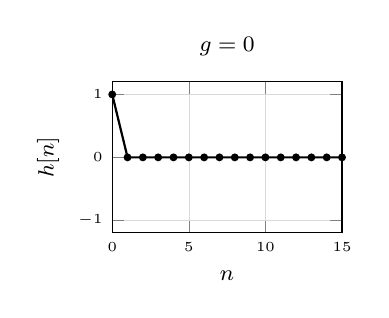
\begin{tikzpicture}
      \begin{axis}[
        width=4.5cm,
        height=3.5cm,
        xlabel={$n$},
        ylabel={$h[n]$},
        xmin=0, xmax=15,
        ymin=-1.2, ymax=1.2,
        grid=major,
        grid style={line width=.1pt, draw=gray!30},
        tick label style={font=\tiny},
        label style={font=\footnotesize},
        title={$g = 0$},
        title style={font=\footnotesize\bfseries}
      ]

      % Risposta con g=0: impulso passa direttamente (feedforward unitario)
      \addplot[
        color=black,
        mark=*,
        mark size=1pt,
        line width=0.8pt
      ] coordinates {
        (0,1) (1,0) (2,0) (3,0) (4,0) (5,0) (6,0) (7,0) (8,0) (9,0) (10,0)
        (11,0) (12,0) (13,0) (14,0) (15,0)
      };

      \end{axis}
    \end{tikzpicture}
    \caption{Passaggio diretto: solo feedforward}
    \label{fig:allpass-zero}
  \end{subfigure}
  \hfill
  \begin{subfigure}[b]{0.32\textwidth}
    \centering
    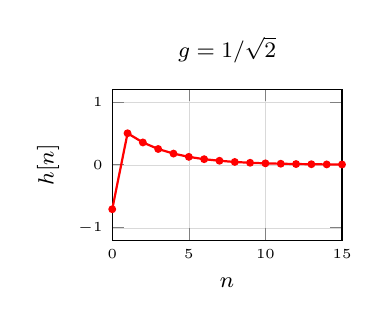
\begin{tikzpicture}
      \begin{axis}[
        width=4.5cm,
        height=3.5cm,
        xlabel={$n$},
        ylabel={$h[n]$},
        xmin=0, xmax=15,
        ymin=-1.2, ymax=1.2,
        grid=major,
        grid style={line width=.1pt, draw=gray!30},
        tick label style={font=\tiny},
        label style={font=\footnotesize},
        title={$g = 1/\sqrt{2}$},
        title style={font=\footnotesize\bfseries}
      ]

      % Risposta AllPass Schroeder corretta con g=1/sqrt(2) ≈ 0.707
      % t=0: -g = -0.707
      % t=τ: (1-g²) = 0.5
      % t=2τ: (1-g²)g = 0.354
      % t=3τ: (1-g²)g² = 0.250
      \addplot[
        color=red,
        mark=*,
        mark size=1pt,
        line width=0.8pt
      ] coordinates {
        (0,-0.707) (1,0.500) (2,0.354) (3,0.250) (4,0.177) (5,0.125)
        (6,0.088) (7,0.063) (8,0.044) (9,0.031) (10,0.022)
        (11,0.016) (12,0.011) (13,0.008) (14,0.005) (15,0.004)
      };

      \end{axis}
    \end{tikzpicture}
    \caption{Equilibrio critico: bilanciamento FIR/IIR}
    \label{fig:allpass-sqrt}
  \end{subfigure}
  \hfill
  \begin{subfigure}[b]{0.32\textwidth}
    \centering
    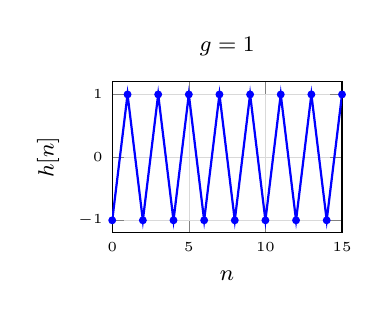
\begin{tikzpicture}
      \begin{axis}[
        width=4.5cm,
        height=3.5cm,
        xlabel={$n$},
        ylabel={$h[n]$},
        xmin=0, xmax=15,
        ymin=-1.2, ymax=1.2,
        grid=major,
        grid style={line width=.1pt, draw=gray!30},
        tick label style={font=\tiny},
        label style={font=\footnotesize},
        title={$g = 1$},
        title style={font=\footnotesize\bfseries}
      ]

      % Risposta AllPass Schroeder con g=1
      % Al limite di stabilità
      \addplot[
        color=blue,
        mark=*,
        mark size=1pt,
        line width=0.8pt
      ] coordinates {
        (0,-1) (1,1) (2,-1) (3,1) (4,-1) (5,1) (6,-1) (7,1)
        (8,-1) (9,1) (10,-1) (11,1) (12,-1) (13,1) (14,-1) (15,1)
      };

      \end{axis}
    \end{tikzpicture}
    \caption{Stallo oscillatorio: dominanza IIR}
    \label{fig:allpass-one}
  \end{subfigure}

% Caption rivisto per i subplot con riferimenti specifici al processo ποίησις
\caption{Dinamiche del processo ποίησις attraverso il filtro AllPass di Schroeder al variare del parametro $g$. ~~~ a) Con $g=0$: la πρᾶξις opera senza memoria teorica, producendo azioni immediate ma prive di risonanza culturale ($H(z) = 1$). ~~~ b) Con $g=1/\sqrt{2} \approx 0.707$: si realizza l'equilibrio creativo aristotelico dove la ποίησις emerge dal bilanciamento dinamico tra πρᾶξις immediata (impulso $-g$ a $t=0$) e θεωρία accumulata (echi decrescenti $(1-g^2)g^n$). ~~~ c) Con $g=1$: la θεωρία domina completamente, il pensiero si cristallizza in pura speculazione senza capacità generativa.}
\label{fig:poiesis-allpass}
\end{figure}


\clearpage

\section{\emph{théatron}: luogo riverberante}

Il greco antico ha diversi termini che esprimono concetti analoghi al
\textit{torquēre} come \textgreek{τρέπω} (trepō), “girare, volgere, cambiare
direzione”. Tuttavia, per il concetto specifico di \emph{torcere con una forza},
quindi “torcere, girare, rivolgere” si usa il verbo \textgreek{στρέφω}
(strephō) da cui deriva il sostantivo \textgreek{στροφή} (strophē), “rotazione,
torsione, volta”, da cui deriva il nostro “strofa”.

La radice di στρέφω è indoeuropea **streb(h)- "torcere", diversa da **terkʷ- ma
semanticamente affine\footnote{La distribuzione del campo semantico su più radici, ciascuna con sfumature
specifiche potrebbe arricchire la riflessione sulla “torsione” come gesto
ermeneutico che si articola in modalità differenti.}.

Quindi “strofa” deriva da “torcere, girare” e designava originariamente il
movimento fisico del coro nella tragedia greca: la “volta” che i coreuti
compivano spostandosi da destra a sinistra nell'orchestra.

La sequenza rituale era: \textgreek{στροφή} (strofe) – movimento verso sinistra;
\textgreek{ἀντιστροφή} (antistrofe) - movimento di ritorno verso destra;
\emph{ἐπῳδός} (epodo): stasi al centro.

Il termine poetico "strofa" conserva questa memoria cinetica: ogni strofa è una
“volta”, un movimento che torna su se stesso, una torsione del discorso che si
riavvolge prima di procedere. La poesia non procede linearmente come la prosa,
ma avanza per spirali, per ritorni, per riprese tematiche. La strofa è la
cellula di questo movimento tortile del senso. In termini filosofici, la
torsione poetica opera quella che Heidegger chiamava \emph{Kehre} - la svolta
che non è semplice cambio di direzione, ma ripiegamento che apre nuove
possibilità di senso. La poesia “torce” il linguaggio ordinario, lo sottopone a
una tensione che ne rivela potenzialità latenti. Così la “torsione filosofica”
dell'oggetto musicale condivide con la poesia questo gesto fondamentale di
deviazione creatrice.

\begin{quote}
\begin{sf}
\small
\ldots spazi vuoti pronti a venirsi riempiendo uno alla volta, spazi della voce
nei quali si apprenderà con l'udito\ldots~\cite{zambrano1991}
\end{sf}
\end{quote}

Il \emph{théatron} messo in piedi per (\emph{theáomai}) questa torsione è un
teatro acustico, poiché la regione in cui si sta organizzando l'assedio è la
conoscenza dell'udire. È sì che si torce: \emph{theōría}: guardare, osservare e,
anche, il risultato di tutto ciò: ma a occhi chiusi, spegnendo l'immagine.
\emph{Theáomai} sì, ma spettatore di altra natura, di altro \emph{théatron}.
Della visione attenta, della contemplazione, tratteniamo la postura, la
partecipazione intellettuale. Come \emph{theōroi}, osservatori ufficiali inviati
ad assistere alla festa del suono, a consultare l'oracolo che chiamiamo musica,
a riferirne ciò ch'è stato udito, sentito, appreso.

L'osservare con le orecchie è a sua volta una torsione, una con-torsione
(dialettica) dell'ascoltare nelle due direzioni opposte e convergenti dell'udire
e del sentire.

\begin{figure}[htbp]
\begin{center}
\begin{tikzpicture}
  \tikzstyle{every node}=[font=\small]
  \ciclodiagram{ascoltare}{udire}{sentire}
\end{tikzpicture}
\caption{L'udire prende il posto della resistenza, la resistenza meccanica si
traduce in una resitenza acustica (impedenza): il materiale risponde alle
sollecitazioni vibrazionali accogliendo, respingendo, ignorando. L'udito è già
selettivo di questa selezione: ha le sue soglie. Resiste e amplifica, è un
sistema di resistenze differenziali. Udire (\emph{Audire}) e anche un obedire
(\emph{Ob-audire}, udire verso). Sentire, connesso a \emph{sensus} e alla radice
indoeuropea \emph{sent-} (“andare, dirigersi”) il sentire è movimento orientato,
direzionalità dell'esperienza. Come \emph{tendere} è “pro-tendersi verso”,
sentire è “dirigersi verso” - entrambi esprimono tensionalità, orientamento
intenzionale.}
\label{ascoltare}
\end{center}
\end{figure}

Lo spazio agonistico \cite{ronchi2001} di questo ascoltare (\emph{theōría}) è
uno spazio della vibrazione acustica udibile, un tempo della vibrazione, uno
spazio dei suoni: un \concetto{sonario}.

\begin{quote}
\begin{sf}
\small
  Io credo che questo doppio movimento di disseminazione e di riunificazione
  semantica sia consustanziale alle nostre lingue e che soltanto attraverso
  questo gesto contraddirorio una parola possa realizzare il suo significato.
  \cite{agamben17}
  \end{sf}
\end{quote}

\apfc{sonario}{impressione}{codice}

Il \emph{sonario} è il nucleo di memoria, di esperienza, in cui si rappresenta
l'im-pressione acustica (della variazione di pressione acustica che si dissemina,
si disperde) e la costruzione di un codice (come sforzo di riunificazione con
la vibrazione perduta).

\begin{figure}[htbp]
\begin{center}
\begin{tikzpicture}
  \tikzstyle{every node}=[font=\small]
  \ciclodiagram{sonario}{impressione}{codice}
\end{tikzpicture}
\caption{}
\label{sonario}
\end{center}
\end{figure}



 il doppio movimento tra
%-------------------------------------------------------------------------------
%----------------------------------------------------------------- SUB-SECTION -
%-------------------------------------------------------------------------------
%\clearpage
\subsection{simbolario intergalattico per autostoppisti}
%\subsection{feedback: creatività, ciclo base}

Percorrere la lunga storia della fantasia creativa occidentale, da Aristotele a
Fagioli \cite{mf:istinto}, con un paio di soste lunghe nei pressi di
Bergson \cite{bergson1896} e Sartre \cite{jps:immaginario}, attraverso le questioni
musicali lucidamente illustrate da Cacciari \cite{Cacciari1995}, ha prodotto un
risultato inatteso, un'assenza: non ho \emph{alternative sonore} alle parole
immaginazione e immaginario; non ho un lessico indipendente dalla visione,
autonomo dal visibile per ciò che conctraddistingue la \emph{fantasia sonora};
l'immaginazione, l'immaginario, spesso si sostituiscono generalizzando fantasia
e creatività, amplificando l'assenza di una parola indipendente e necessaria per
l'attività creatrice sonora.

\begin{quote}
\begin{sf}
\small
Gli uomini medievali non provavano fiducia per i loro sensi; l'orecchio musicale
non offriva sufficiente sicurezza. Il metodo scolastico degli studiosi non
includeva la ricerca e l'esperimento, ma consisteva nel trovare una autorità
classica e nell'adottare le sue conclusioni riguardo a problemi contemporanei.
Certamente dal greco Aristosseno i musicisti medievali avrebbero potuto
apprendere il rispetto per l'orecchio musicale, ma proprio a causa di questa
fiducia nelle impressioni sensoriali egli era rifiutato dai monaci; uno
scrittore anonimo, probabilmente dell'XI secolo, affermò ingenuamente che Boezio
non sarebbe mai andato d'accordo con Aristosseno... \cite{sachs1996}
\end{sf}
\end{quote}

Si vuole raccontare una storia. Al fianco del \emph{vedere-comprendere} che
riflette la concezione classica della conoscenza come visione intellegibile che
pervade tutto il vocabolario epistemologico occidentale (idee, evidenza,
intuizione, immaginazione\ldots) la storia che si vuole raccontare ha origini
antichissime, come la visione, con lo stesso dualismo dialettico agonistico tra
teorico e pratico, con lo stesso eterno desiderio di giungere alla \emph{theōría}
con quel significato tecnico scientifico di sistema coerente di principi che
spiegano un insieme di fenomeni. Così, si vuole raccontare una storia %dell'esperienza musicale.

\begin{quote}
\begin{sf}
\small
we have to perceive what is coming to be and remember what has come to be. There
is no other way of following the contents of music\footnote{Aristosseno, Elementa
Harmonica, book II, 38–39. Traduzione in \emph{The Stanford Encyclopedia of
Philosophy}}
\end{sf}
\end{quote}

Mi pare che Aristosseno attivi, come il suo Maestro Aristotele, quell'\emph{agōn}
\cite{ronchi2001} tra sensazione (volpe – «pura inafferrabilità») e memoria (cane
– «pura potenza dell'afferrare»); costituisce quel «per sempre avere luogo» nella
rappresentazione istantanea, nella coesistenza tra sensazione e memoria che
chiamiamo \emph{esperienza musicale}.

Ascoltare mediante l'ascolto musicale è un passare attraverso il “foro” della
musica: oltrepassa la soglia solo un qualcosa, in un certo modo.

\vspace{1cm}

DIFFRAZIONE

«\ldots perceive what is coming» è una postura, una modalità su cui il modo della
vibrazione acustica si schianta, si riflette, si incide in negativo.

\vspace{1cm}

NEGATIVO SEGNO RONCHI

Si fa traccia dell'assoluto suono. Questo svolgersi è un processo inverso,
specchiato, di ingranaggi che ruotano in sensi opposti, cedendosi informazioni
inverse. Ci si timbra, ascoltando, con l'ascolto.

La storia, quindi, sottolinea la dimensione temporale della coscienza musicale,
ovvero la percezione di ciò che \emph{è diventato} (orientata al passato) e il
ricordo di ciò che \emph{sta per diventare} (orientato al futuro).

\begin{figure}[htbp]
\begin{center}
\begin{tikzpicture}
  \tikzstyle{every node}=[font=\small]
  \ciclodiagram{coscienza musicale}{sensazione}{memoria}
\end{tikzpicture}
\caption{Ciò che in Aristosseno è \emph{pre}-disposizione per l'esperienza
musicale, si ri-organizza all'\emph{inverso} \cite{bergson:segno} nella coscienza
di quella esperienza con la sensazione uditiva di una vibrazione che per
definizione è già passata; la memoria di quel passato è protesa ad un nuovo futuro.}
\label{coscienza}
\end{center}
\end{figure}

Penso suoni, ricordo suoni, (\emph{sogno suoni?}) e più mi impegno nel farlo e
più trovo che l'attività che faccio abbia poco a che vedere con l'immaginazione;
l'attività creativa di \emph{sonazione}, di invenzione timbrica, di messa a
punto di una tecnica d'indagine estesa dentro gli strumenti musicali
\cite{netti23} conduce alla costruzione di un \emph{sonario} rappresentabile sia
nel processo di scrittura (in funzione di riduzione simbolica) sia nella
relazione di dialogo possibile ed esclusivo tra musicisti.

\begin{description}
  \item[Glossario] Dal latino tardo \emph{glossarium}, derivato da \emph{glossa}
  (parola rara o straniera che necessita spiegazione), a sua volta dal greco
  \textgreek{γλῶσσα} (glōssa) che significa "lingua" o "linguaggio". Raccolta di
  termini specifici di una disciplina, ordinati alfabeticamente e corredati di
  definizione. Originariamente era una raccolta di termini difficili o arcaici
  (\emph{glossae}) con relative spiegazioni.
  \item[Immaginario] Dal latino \emph{imaginarius} (che esiste solo
  nell'immaginazione), derivato da \emph{imago, imaginis} (immagine,
  rappresentazione), connesso alla radice indoeuropea \emph{im-} (copiare,
  imitare). Come sostantivo, indica l'insieme delle immagini, dei simboli e
  delle rappresentazioni mentali condivise da una cultura o da un individuo. È
  il luogo concettuale dove risiedono le immagini che costituiscono il nostro
  modo di vedere e interpretare il mondo.
  \item[Scenario] Dal tardo latino \emph{scenarium}, derivato da \emph{scena}
  (palcoscenico, scena teatrale), che proviene dal greco \textgreek{σκηνή}
  (skēnē), originariamente "tenda, riparo" poi "palcoscenico". Inizialmente
  indicava l'insieme delle scene di una rappresentazione teatrale. Per
  estensione, oggi denota la descrizione di una possibile sequenza di eventi o
  sviluppi futuri, o l'ambientazione in cui si svolge un'azione.
\end{description}

Come il glossario raccoglie e definisce le parole, l'immaginario accoglie e
struttura le immagini, lo scenario esemplifica lo spazio delle scene, sia esso
verticale (coesistenza) che orizzontale (successione) così il \emph{sonario}
diventa il ricettacolo ontologico dei fenomeni sonori, in relazione all'ascolto,
alla creazione e alla riflessione umana.

\begin{description}
  \item[Sonario] Dal latino \emph{sonus} (suono) con il suffisso \emph{-arium}
  che indica raccolta, contenitore o luogo dedicato. Il \emph{Sonario} è lo
  spazio agonistico della ragione acustica che si fa metodo nella coscienza
  musicale, il \emph{théatron} dove il suono si fa interfaccia teorico-pratica –
  dove \textgreek{θεωρία}, \textgreek{πρᾶξις} e \textgreek{ποίησις} si dispiegano.
\end{description}

Il termine “simbolario” deriva dal latino “symbolum” (che a sua volta viene dal
greco \textgreek{σύμβολον} (symbolon), letteralmente “segno di riconoscimento”)
e indica una raccolta sistematica di simboli con i loro significati\footnote{Nel
contesto della segnaletica stradale, il simbolario costituisce l'insieme
codificato di tutti i pittogrammi, ideogrammi e simboli grafici utilizzati nella
comunicazione visiva del traffico.}.

L'insieme codificato di tutti i simboli costituisce un codice e, in quanto tale,
opera su due livelli semiotici:
\begin{description}
  \item[il livello simbolico immediato]: il sistema di segni visivi che
  comunicano direttamente attraverso la percezione, sfruttando convenzioni
  iconografiche universali;
  \item[il livello normativo mediato]: l'apparato di regole scritte che
  richiedono interpretazione linguistica e conoscenza giuridica per essere
  applicate.
\end{description}

Questa dualità riflette due modalità cognitive diverse: il riconoscimento
immediato (quasi istintivo) versus la comprensione mediata dal linguaggio e
dalla memoria delle norme.

“Codice” deriva dal latino \emph{codex} (genitivo \emph{codicis}), che
originariamente significava “tronco d'albero” o “pezzo di legno”.

Il passaggio da “tronco” a “sistema di regole” attraversa la materialità del
supporto scrittorio: dal legno come materia prima alla scrittura come
codificazione del sapere normativo. C'è quasi una genealogia che va dalla natura
(albero) alla cultura (diritto), mediata dalla tecnica della scrittura.

La parola mantiene oggi questa tensione tra materialità e astrazione: un codice
è insieme supporto fisico e sistema logico.

\begin{quote}
\begin{sf}
\small
  Una classificazione è sempre una sintomatologia e ciò che viene classificato
  sono dei segni, per tirarne fuori un concetto che si presenta come un evento,
  non come un'essenza astratta. Da questo punto di vista le varie discipline
  sono veramente delle materie segnaletiche.
  \cite{deleuze2009}
  \end{sf}
\end{quote}

\begin{quote}
\begin{sf}
\small
  Il cinema non va compreso come un linguaggio, ma come una materia segnaletica.
  \cite{deleuze2009}
  \end{sf}
\end{quote}


%-------------------------------------------------------------------------------
%----------------------------------------------------------------- SUB-SECTION -
%-------------------------------------------------------------------------------
\subsection{creatività e allucinazione}

Una definizione di allucinazione indica un «\emph{fenomeno} psichico,
provocato da cause diverse, per cui un individuo percepisce come reale ciò che
è solo \emph{immaginario}.» Immaginario, «che è \emph{effetto} d'immaginazione»
in contrapposizione con reale, «che è, che \emph{esiste effettivamente} e
concretamente, non illusorio, immaginario o possibile». Quindi il reale non è
possibile, in quanto reale, mentre l'immaginario può essere possibile.

\begin{quote}
  La possibilità non è la realtà, ma è anch'essa una realtà: che l'uomo possa
  fare una cosa o non possa farla, ha la sua importanza per valutare ciò che
  realmente si fa. Possibilità vuol dire libertà. \cite{ag:matst}
\end{quote}% GRAMSCI P35

L'immaginario può essere possibile; possibilità vuol dire libertà: la creatività,
libera, è un percorso di trasduzione da un'informazione immaginaria a
un'informazione possibile: un processo possibile dall'idea alla cosa.

Ma l'immaginario, quando collettivo, è anche una cosa, un \emph{insieme di
simboli e concetti presenti nella memoria} di una comunità: una memoria
collettiva. L'\emph{insieme di rappresentazioni simboliche}.

Quindi la creatività libera e contemporanea \cite{agamben08} del singolo
(quella possibile, immaginaria, inattuale) si stacca dall'immaginario collettivo
che è fondamentalmente memoria, passato, passato di altri, in una forma di
rappresentazione privata, in attesa di condivisione, in attesa forse di divenire
memoria collettiva di altri, di un altro tempo.

\begin{quote}
  Il punto cioè in cui la concezione del mondo, la contemplazione, la filosofia
  diventano «reali» perché tendono a modificare il mondo, a rovesciare la prassi.
  \cite{ag:matst}
\end{quote}% GRAMSCI P41

L'allucinazione è anche descritta come \emph{turbamento mentale}, come la
comparsa di \emph{immagini sensoriali} dotate di \emph{piena evidenza realistica},
che vengono posizionate, inquadrate, viste, udite, sentite, come sensazioni,
nella realtà esterna, formate, tuttavia, per un processo interno, anche in
assenza o senza che sia presente, o esista, l'oggetto o il fatto corrispondente.

\begin{quote}
  Creativo, occorre intenderlo quindi nel senso «relativo», di pensiero che
  modifica il modo di sentire del maggior numero e quindi la realtà stessa che
  non può essere pensata senza questo maggior numero. Creativo anche nel senso
  che insegna come non esista una «realtà» per se stante, in sé per sé, ma in
  rapporto storico con gli uomini che la modificano, ecc\ldots \cite{ag:matst}
\end{quote}% GRAMSCI P23

Per portare questo quadro, questa diagnosi, all'interno del processo creativo
sonoro, accedere alla rappresentazione, quindi alla \emph{sonazione} nella
costruzione di un \emph{sonario} personale e condivisibile è necessario
soffermarsi sul sensibile, sugli oggetti che dall'ambiente diventano coscienza,
a volte conoscienza.

Come suggerisce Domenico Guaccero \cite{branchi1977tecnologia} riparto
dall'osservazione dei fenomeni cercando la relazione organica con
l'ambiente, nel tentativo di condividere un primo prototipo di \emph{sonario}.
Il fenomeno sotto osservazione è la vibrazione acustica, quella particolare
vibrazione che rientra nell'ambito multidimensionale\footnote{%
  Un fenomeno acustico è udibile se soddisfa tutte e tre le dimensioni: tempo,
  ampiezza, frequenza.
} dell'udibile: la vibrazione è udibile, energia potenziale. Il fenomeno fisico
è esterno, e l'organo dell'udito è l'entrata, verso l'interno dell'uditore.
Fuori da quell'ambito c'è l'inudibile, dentro quell'ambito c'è l'udibile. Il
grado successivo di intimazione è il sentire: non si è più fuori, si è già
dentro l'organo di senso.

\begin{quote}
  Il senso in musica è l'interfaccia uomo/musica. \cite{stefani}
\end{quote}

La vibrazione sensibile, dentro e dopo le soglie di udibilità, entra in
relazione con la sensibilità individuale. È quello che nel senso comune
chimiamo suono, la rappresentazione della vibrazione acustica.

Il suono non è la vibrazione stessa ma il residuo di quella sensazione specifica
di quella vibrazione acustica. Non è fuori, ma dentro. È esperienza, quindi
memoria, quindi coscienza. Mentre la vibrazione è attivazione del meccanismo
uditivo, il suono è un'esperienza della mente. Questo apre ad una soglia
invalicabile: il silenzio è l'esperienza inaccessibile. La non-esperienza che
attrae e che apre ad altre esperienze (sonore). Luigi Nono, John
Cage\ldots~nuovi suoni in cerca di silenzio, verso nuove musiche: il suono
diviene storia del suono, storia del silenzio, storia della musica.

Nella meccanica del reale esperibile la coordinata temporale è inevitabile.
L'esperienza è nel tempo. Il tempo è esperienza. Se è presente la coordinata
temporale non può essereci silenzio. \emph{Il silenzio non esiste} novecentesco
è vero solo se ci si attiene alla meccanica tradizionale e al reale percepibile.
Tuttavia, il silenzio può esistere nelle strutture mentali e quindi nella fisica
quantistica, ovvero là dove la coordinata temporale smette di avere quel
significato. Potrei così giocare con il linguaggio: il silenzio è così
allusivamente attraente, relazionale, perché è quantistico. Il legame tra parola
e tempo ci pone nel dominio meccanico del dire, conducendo la parola, a volte
frammenti di essa, nel luogo senza tempo della relazione, si entra nel dominio
quantistico della poesia.

Tornando al sistema di riferimento musicale, il silenzio è nelle relazioni tra i
suoni, a cui tendiamo prima e dopo di ognuno di questi. La soglia che separa
l'uomo sensibile dal silenzio è una curva di ampiezze dipendenti dalla frequenza
nel tempo: un sistema musicale: in un sistema fisico: in un sistema filosofico.

\emph{E il rumore?} Il rumore è semplicemente la vibrazione di cui non si ha
ancora esperienza. La vita del rumore è la durata, la transizione, tra silenzio
ed esperienza.

Tendere a quella soglia ci porta a scoprire nuovi suoni, perfetti sconosciuti:
rumori. Siamo ascoltatori di uno spazio esteso oltre il conosciuto, come un
Galileo al tubo ottico: cerchiamo cose, per sentirne alcune, per udirne
altre, per dare nomi, per creare relazioni. Pionieri della \emph{sonazione}.

\begin{quote}
  [\ldots] l'unità di scienza e vita è appunto una unità attiva, in cui solo si
  realizza la libertà di pensiero, è un rapporto maestro-scolaro,
  filosofo-ambiente culturale in cui operare, da cui trarre i problemi necessari
  da impostare e risolvere, cioè il rapporto filosofia-storia. \cite{ag:matst}
\end{quote}% GRAMSCI P22

% $vibrazione(acustica) + esperienza(tempo) + spazio = timbro$. L'orecchio:
% strumento millenario, perfezionato per scappare e predare. Utilizzato come luogo
% creativo in cui costruire strumenti artificiali, l'orecchio, apre a nuove
% parole: Timbro. Quando predavamo scappando dai predatori non esisteva il
% timbro. Ci sono voluti secoli di strumenti artificiali, oggetti che hanno
% permesso una storia della musica, di tecnica e pensiero, per avere necessità di
% una nuova parola.
%
% Attività creativa, creazione come luogo particolareggiato del fare umano.
% Lo strumento come strumento di pensiero e la necessità di nuovi strumenti di
% pensiero.

L'allucinazione \emph{sonaria} è quindi una rappresentazione unica, ideale fino
a che non viene concessa e condivisa con una seconda persona: l'idea di un
singolo, privata agli altri, non è un oggetto sociale, mentre un'allucinazione
\emph{sonaria} condivisa e comprensibile è un oggetto sociale: è un possibile.
\cite{ferraris2014}
%-------------------------------------------------------------------------------
%----------------------------------------------------------------- SUB-SECTION -
%-------------------------------------------------------------------------------
\subsection{allucinazione e sogno}

Il motore che anima la ricerca è il sogno. Ogni scienza è guidata da un sogno.
Il sogno è l'anima della scienza, ogni scienza si distingue nella prospettiva di
un sogno: la ricerca di quel sogno specifico è lo spirito di quella scienza.
(Da Bergson) Il pensiero filosofico è tornato co-scienza della scienza. La
materia è memoria: la musica è un'interfaccia tecnologica della memoria.

\begin{quote}
  Non c’è, nella ragione del logos la linea che è creazione pura. La
  simbolizzazione della scrittura non può essere neppure trasformazione di una
  cosa percepita, ovvero immagine onirica, perché la linea, fuori ed oltre la
  mano dell’uomo che la segna, non esiste in natura e non può essere percepita
  e fatta ricordo o memoria. Noi percepiamo la linea che non ha figura ed ha
  forme infinite ed è senza identità manifesta, per la creazione della mano
  dell’uomo che fa i confini e definisce, rendendole visibili, le forme e la
  figura delle cose e delle immagini delle cose. E così crea anche l’identità
  della linea stessa che, ogni volta, è diversa perché infinitamente sottile o
  infinitamente lunga. E penso alla parola tempo che indica un movimento che
  non si ferma mai e non ha figura, né forma né confini. Ma il movimento
  invisibile della materia vivente non possiamo vederlo. Linea, movimento e
  tempo sono ancora tre parole che non indicano e non ricordano la figura
  di una cosa, ma sono... concetti, l’espressione di cose invisibili che si
  possono soltanto pensare. \cite{mf:left2008}
\end{quote}

La spiegazione del processo creativo che \emph{Cobb} condivide con
\emph{Ariadne}, del potenziale mentale nel sogno, è una delle tematiche
emergenti in \emph{Inception}, durante la cui scrittura l'autore, Christopher
Nolan, si è chiesto: «cosa accadrebbe se un gruppo di persone potesse
condividere (realmente) un sogno?».

\begin{figure}[ht]
\centering
%\resizebox{0.81\linewidth}{!}{%
%\includegraphics[scale=1]{tikz/inception/inception.pdf}
\begin{tikzpicture}
  \tikzstyle{every node}=[font=\small]
  \ciclodiagram{}{}{}
\end{tikzpicture}
%\captionsetup{width=.81\linewidth}
\caption{Christopher Nolan, \emph{Inception} (2010).\\
         «Imagine you're designing a building. \textbf{You consciously create
         each aspect}. But sometimes,
         \textbf{it feels like it's almost creating itself}, if you know what I
         mean». «Yeah, like \textbf{I'm discovering it}». «Genuine inspiration,
         right? Now, in a dream, our mind continuously does this.
         \textbf{We create and perceive our world simultaneusly}. And our mind
         does this so well that we don't even know it's happening.
         \textbf{That allows us to get right in the middle of that process}».
         «How?». «\textbf{By taking over the creating part}».
         Il grafico disegnato da Cobb descrive il processo creativo di un sogno
         durante la costruzione di un edificio. Nel sogno, la curva che avanza
         da sinistra verso destra è il lavoro di costruzione che avanza mentre
         la curva che torna indietro da destra verso sinistra è la percezione,
         la scoperta di un mondo che si crea da solo. La riga centrale è «la
         presa in carico della parte creativa», la consapevolezza che si sta
         creando su due piani distinti.}
\label{tikz:inception}
\end{figure}

Il disegno in fig. \ref{tikz:inception} ricalca quello proposto da \emph{Cobb}
durante la spiegazione citata.
Osservandolo, mi chiedo: «non è quello che (simbolicamente) accade nella
condivisione di una ricerca?» L'attività creativa, quella che Fagioli definisce
creazione pura, non ha origini dal percepito, si attiva, è attività di
costruzione, di architettura, di autoprogettazione.

\begin{figure}[ht]
  \centering
  \begin{tikzpicture}
    \tikzstyle{every node}=[font=\small]
    \ciclodiagram{creatività}{invenzione}{ricerca}
  \end{tikzpicture}
  %\includegraphics{tikz/ciclo-base/ciclobase.pdf}
  %\captionsetup{width=.81\linewidth}
  \caption{ciclo base: l'invenzione è il trovato; la ricerca è coscienza protesa
  fuori dal tempo. L'atto creativo è un momento di ebaborazione della memoria che
  modifica l'ambiente.}
  \label{tikz:ciclobase}
\end{figure}

Il processo è trasducibile completamente nel dominio della creazione musicale,
la consapevolezza creativa, l'atto responsabile è l'asse su cui l'invenzione
avanza verso destra, nel dominio del tempo, mentre la ricerca si muove fuori
dal tempo, nello spazio mentale di relazione con la storia e l'ambiente.
Il disegno è simbolico del puro processo creativo, sogno o arte.
%
% \marginpar{%
%   \includegraphics[width=\marginparwidth]{images/apf.png}
%   \captionof{figure}{\raggedright Diagramma di un filtro \emph{all-pass}.}
%   \label{img:apf}
% }
%
Osserviamo ora il diagramma della creazione: è un ciclo base tra l'invenzione,
il trovato nella relazione con l'ambiente e la pulsione di ricerca, con le sue
possibilità fuori del tempo e che modificano l'ambiente ri-alimentandolo con un
apparato di idee e materia completamente nuovi. Di fatto, se contempliamo il
processo creativo come quel flusso temporale in cui ci si può perdere un tempo
di sedimentazione, di accumulazione (come una pausa caffè e sigaretta) il
modello descritto è astraibile ad un filtro \emph{all-pass}. Nella letteratura
classica il filtro \emph{all-pass} viene descritto come unità riverberante. Il
processo creativo di relazioni intime, private, in una rete di relazioni tra
processi creativi può essere descritto come riverbero complesso, assimilabile
ad una \emph{Feedback Delay Network}.

%-------------------------------------------------------------------------------
%----------------------------------------------------------------- SUB-SECTION -
%-------------------------------------------------------------------------------
\subsection{sogno e politica}

\begin{quote}
  Che cos'è l'uomo? %È questa la domanda prima e princicpale della filosofia.
  [\ldots] Diaciamo dunque che l'uomo è un processo e precisamente è il
  processo dei suoi atti. [\ldots] occorre concepire l'uomo come una serie di
  rapporti attivi (un processo) in cui se l'individualità ha la massima
  importanza, non è però il solo elemento da considerare. L'umanità che si
  riflette in ogni individualità è composta di diversi elementi: 1) individuo;
  2) gli altri uomini; 3) la natura. [\ldots] Così l'uomo non entra in rapporti
  con la natura semplicemente per il fatto di essere egli stesso natura, ma
  attivamente, per mezzo del lavoro e della tecnica [\ldots] per tecnica deve
  intendersi [\ldots] anche gli strumenti «mentali», la conoscenza filosofica.
\end{quote}% GRAMSCI P27-28

È questo, innanzi tutto, un problema di linguaggio. Con linguaggio identifichiamo
un nome collettivo, che non presupone una cosa unica, è un \emph{oggetto sociale}.
\cite{ag:matst, ferraris2014} Esiste nella cultura, nella filosofia e nella
scienza, sia pure nel grado di senso comune e, in quanto tale, è una
molteplicità di oggetti, fatti, più o meno organicamente concreti e coordinati:

\begin{quote}
  al limite si può dire che ogni essere parlante ha un proprio linguaggio
  personale, cioè un proprio modo di pensare e sentire. \cite{ag:matst}
\end{quote}

E quindi la cultura unifica, raggruppa, cataloga a sua volta una maggiore o
minore quantità di individui più o meno a contatto espressivo, capaci di gradi
diversi di comprensione. Le differenze si riflettono, si riverberano nella
cultura, nel linguaggio comune e producono «ostacoli» e quelle «cause di errore»
che portano, da un lato all'incomprensione, dall'altro alla separazione, in
ogni caso riverbera in un problema ambientale. La conoscenza non è separata e
sufficiente a sé stessa, ma è coinvolta nella relazione individuo-ambiente e
nel processo culturale, vitale. I sensi non appaiono come ingressi della
conoscenza ma partecipano come stimoli all’azione.

\begin{quote}
  \ldots ognuno cambia se stesso, si modifica, nella misura in cui cambia e
  modifica tutto il complesso di rapporti di cui egli è il centro di annodamento.
  In questo senso il filosofo reale è e non può essere altri che il politico,
  cioè l'uomo attivo che modifica l'ambiente, inteso per ambiente l'insieme dei
  rapporti di cui ogni singolo entra a far parte. %Se la propria individualità
  %è l'insieme di questi rapporti, farsi una personalità significa acquistare
  %coscienza di tali rapporti, modificare la propria personalità significa
  %modificare l'insieme di questi rapporti.
  [\ldots] Ma questi rapporti, come si è detto, non sono semplici. Intanto
  alcuni di essi sono necessari, altri volontari. Inoltre averne coscienza più
  o meno profonda (cioè conoscere più o meno il modo con cui si possono
  modificare) già li modifica. Gli stessi rapporti necessari in quanto
  conosciuti nella loro necessità, cambiano d'aspetto e d'importanza.
  La conoscenza è potere in questo senso. \cite{ag:matst}
\end{quote}% GRAMSCI P29

Se la musica ha avuto ed ha un ruolo culturale fuori dall'intrattenimento, è
in questi \emph{non}-spazi e in questi \emph{non}-tempi sociali. Se il musicista
ha ancora un ruolo sociale fuori dall'intrattenitore è in questi spazi e in
questi tempi culturali. Ridefinire il proprio ambito di intervento culturale e
sociale implica una concertazione, un accordo in maniera che la meta della
ricerca sia il risultato di un’appropriata combinazione di accordo non
costrittivo e tollerante disaccordo.

\begin{quote}
  Secoli e secoli di idealismo non hanno mancato di influire sulla realtà. \cite{jlb:finzioni}
\end{quote}% BORGES

\begin{quote}
\begin{sf}
\small
  “Autore” è una funzione ce rinvia all'opera d'arte (e in altre condizioni al
  crimine).
  \cite{deleuze2009}
  \end{sf}
\end{quote}


\clearpage

\section{«\ldots del loro oggetto»: \emph{per quale musica?}}

\emph{Theōría}, l'attività d'osservazione attenta e contemplativa (in musica:
\emph{ascolto}) che si relaziona con la \emph{praxis} condotta strumento alla
mano, come questa penna stilografica, e che adduce alla \emph{poiesis}: la musica.

Per Aristotele questo spazio agonistico è tripartito in \emph{bios theoretikos,
bios praktikos, bios poietikos}. All'interno della visione di questa
\emph{theōría} diviene

\begin{figure}[htbp]
\begin{center}
\begin{tikzpicture}
  \tikzstyle{every node}=[font=\small]
  \ciclodiagram{ποίησις}{πράξις}{θεωρία}
\end{tikzpicture}
\caption{Il processo aristotelico della ποίησις emerge dalla tensione dinamica
tra pratica (πρᾶξις) e teoria (θεωρία), realizzando un ciclo temporale dove ogni
elemento si alimenta degli altri senza perdita di energia com- plessiva. Questo
movimento circolare rappresenta l’isomorfismo fondamentale con il filtro AllPass:
conservazione dell’energia informazionale attraverso trasformazione delle
relazioni temporali.}
\label{poiesis}
\end{center}
\end{figure}

In questo spazio vorrei approfondire alcune problematiche che emergono dalla lettura del primo capitolo del Manuale di Armonia di Schoenberg (riportato in appendice) \cite{schonberg1970} in relazione a ciò che è emerso nella seconda metà del secolo (evangelisti).

\begin{quote}
\begin{sf}
\small
  Le altre pratiche (pittura, fotografia, cinema, ecc.) sono chiamate in causa
  solo al prezzo di una preliminare torsione filosofica del loro oggetto.
  \cite{ronchi2001}
  \end{sf}
\end{quote}

Qual è l'oggetto della musica? Mi viene alla memoria il domandare, domandandosi,
di Deleuze in \emph{Che cos'è l'atto di creazione?} \cite{deleuze2009} Ci-si
chiede «cosa faccio io quando faccio o spero di fare filosofia?». È una
conferenza, si rivolge agli studenti «che cosa fate voi che fate cinema?» E poi
«che cos'è avere un'idea al cinema?»

\begin{quote}
\begin{sf}
\small
  Le idee bisogna considerarle come dei potenziali già impegnati in questo o in
  quel modo d'espressione e inseparabili dal modo d'espressione\ldots In funzione
  delle tecniche che conosco posso avere un'idea in un certo ambito\ldots
  \cite{deleuze2009}
  \end{sf}
\end{quote}

Per avvicinarmi al «loro oggetto» e distinguerlo dalla torsione filosofica devo
passare per «che cos'è il contenuto della filosofia?»

\begin{quote}
\begin{sf}
\small
  \ldots la filosofia è una disciplina che crea e inventa come le altre. Crea o
  inventa concetti. [\ldots] Ci vuole una necssità, in filosofia come altrove, altrimenti non c'è proprio niente.
  \cite{deleuze2009}
  \end{sf}
\end{quote}

La musica crea dei blocchi di suoni/timbri.

\begin{quote}
\begin{sf}
\small
  Se tutte le discipline comunicano fra di loro è sul piano di ciò che non si
  libera mai per se stesso, ma che è come \emph{impegnato} in ogni disciplina
  creatrice, cioè la costituzione degli spazio-tempo.
  \cite{deleuze2009}
  \end{sf}
\end{quote}

\begin{quote}
\begin{sf}
\small
  Il sogno è una terribile volontà di potenza.
  \cite{deleuze2009}
  \end{sf}
\end{quote}

\begin{quote}
\begin{sf}
\small
  Mi dico che avere un'idea non è comunque dell'ordine della comunicazione.
  [\ldots] Non tutto ciò che di cui si parla è riducibile alla comunicazione.
  [\ldots] la comunicazione è la trasmissione e la propagazione di
  un'informazione. [\ldots] un'informazione è un'insieme di parole d'ordine.
  [\ldots] Non ci viene chiesto di credere, ma di comportarci come se credessimo.
  [\ldots] Ciò significa che l'informazione è proprio il sistema del controllo.
  \cite{deleuze2009}
  \end{sf}
\end{quote}

\begin{quote}
\begin{sf}
\small
  La contro-informazione è effettiva solo quando diventa un atto di resistenza.
  \cite{deleuze2009}
  \end{sf}
\end{quote}

\apf{atto di resistenza}{informazione}{contro-informazione}


\begin{quote}
\begin{sf}
\small
  Che rapporto ha l'opera d'arte con la comunicazione?

  Nessuno. L'opera d'arte non è uno strumento di comuinicazione. L'opera d'arte
  non ha niente a che fare con la comunicazione. L'opera d'arte non contiene
  letteralmente la minima informazione. Cìè invece un'affinità fondamentale tra
  l'opera d'arte e l'atto di resistenza.
  \cite{deleuze2009}
  \end{sf}
\end{quote}

l'opera d'arte

\begin{quote}
\begin{sf}
\small
  Malraux\ldots dice che è la sola cosa che resiste alla morte\ldots l'arte
  è ciò che resiste\ldots
  \cite{deleuze2009}
  \end{sf}
\end{quote}

\begin{quote}
\begin{sf}
\small
  Mpm ogni atto di resistenza è un'opera d'arte, benché, in un certo senso, lo
  sia. Non ogni opera d'arte è un atto di resistenza e tuttavia, in un certo
  senso, lo è.
  \cite{deleuze2009}
  \end{sf}
\end{quote}

\begin{quote}
\begin{sf}
\small
  Non c'è opera d'arte che non faccia appello a un popolo che non esiste ancora.
  \cite{deleuze2009}
  \end{sf}
\end{quote}

\begin{quote}
\begin{sf}
\small
  Un'arte produce invece necessariamente un che di inatteso, di non riconosciuto,
  di non-riconoscibile.
  \cite{deleuze2009}
  \end{sf}
\end{quote}

\begin{quote}
\begin{sf}
\small
  Un'opera è sempre la creazione di un nuovo spazio-tempo\ldots deve far scaturire
  problemi e questioni in cui veniamo presi, piuttosto che dare risposte. Un'opera
  è una nuova sintassi, cosa che è molto più importante del vocabolario, e scava
  una lingua straniera nella lingua.
  \cite{deleuze2009}
  \end{sf}
\end{quote}

\begin{quote}
\begin{sf}
\small
  La novità è il solo criterio dell'opera. Se non si pensa di aver visto
  qualcosa di nuovo o di aver qualcosa di nuovo da dire, perché mai scrivere,
  dipingere o prendere una cinepresa? [\ldots] Il nuovo, in questo senso, è
  sempre l'inatteso, ma anche ciò che diventa immediatamente eterno e necessario.

  \cite{deleuze2009}
  \end{sf}
\end{quote}


\clearpage

\thispagestyle{empty}
\null\vfill
{\Huge\emph{appendici}}
\vfill\null

\clearpage

\appendix
\thispagestyle{empty}

\section{Arnold Schoenberg: Teoria o metodologia?}

Colui che insegna composizione musicale è chiamato insegnante di teoria; chi poi ha scritto un trattato di armonia è chiamato addirittura teorico. Eppure a un falegname, che anch'egli deve insegnare il mestiere al suo apprendista, non verrà mai in mente di spacciarsi per «insegnante di teoria»: semmai si definisce mastro falegname, che è però più designazione di condizione che titolo; e in nessun caso si ritiene qualcosa come un dotto, anche se alla fin fine conosce il suo mestiere. Se esiste una differenza, essa può consistere solo nel fatto che la tecnica della musica è più «teorica» di quella del falegname: il che non è poi cosi ovvio. Il fatto che il falegname sappia come si uniscono solidamente tra loro i diversi pezzi di legno si basa sull'osservazione acuta e sull'esperienza, così come avviene quando il «teorico» musicale sa collegare tra loro con efficacia gli accordi. Se il falegname sa che qualità di legname usare per determinate esigenze è perché valuta i rapporti naturali e del materiale, così come fa il «teorico» musicale quando stabilisce, valutando le possibilità dei temi, la lunghezza che può avere un pezzo di musica. Quando il falegname guarnisce con scannellature una superficie piatta per ravvivarla, anch'egli denota cattivo gusto e poca fantasia al pari di quasi tutti gli artisti, ma sempre in misura non inferiore a quella di un «teorico» della musica. Dunque, l'insegnamento del falegname si basa, come quello dell'insegnante di teoria, sull'osservazione, sull'esperienza, sulla riflessione e il gusto, sulla conoscenza delle leggi naturali e delle proprietà del materiale; ma allora, esiste proprio una differenza sostanziale?

Perché dunque un mastro. falegname non si chiama «teorico», o un teorico della musica «mastro musico»? Perché c'è una piccola differenza: il falegname non dovrebbe mai intendere il suo mestiere da un punto di vista esclusivamente teorico, mentre il teorico musicale in genere non ha nessuna capacità pratica; insomma non è un «mastro». Altra differenza: il vero teorico della musica si vergogna del mestiere, perché non è cosa \emph{sua} ma \emph{di altri}; e non gli basta nascondere questo fatto, senza far di necessità virtù, cosicché il titolo di «maestro» è svalutato, perché potrebbe generare confusione con altri mestieri. Di qui la terza differenza: a una Professione più nobile deve corrispondere un più nobile titolo, e per questo la musica - benché ancor oggi il grande musicista venga chiamato «maestro» - non ha, come persino la pittura, un tirocinio artigianale ma l'insegnamento della teoria.

Conseguenza è che nessun'arte è stata tanto ostacolata nel suo sviluppo dai suoi insegnanti quanto la musica, perché non esiste custode più geloso dei suoi averi di chi sa che essi, in fondo, non gli appartengono: quanto più è difficile dimostrare la legittimità del proprio possesso, tanto maggiore è lo sforzo di procurarsela. Il teorico, che di solito non è artista o è un cattivo artista (che è quanto dire che artista non è), ha tutte le ragioni per darsi da fare a consolidare la sua posizione innaturale. Sa che l'allievo imparerà soprattutto dai modelli che i veri Maestri gli indicano nei loro capolavori; e se gli allievi potessero assistere alla composizione della musica come possono assistere alla nascita di un quadro, se ci fossero studi di composizione come ci sono di pittura, sarebbe allora chiaro che l'insegnante di teoria è superfluo, anzi nocivo, come le accademie d'arte.

Questo il teorico lo avverte, e si cerca un surrogato ponendo la teoria, il sistema, al posto del modello vivo.
Non voglio polemizzare con i tentativi onesti di chi cerca di trovare le presunte leggi dell'arte: essi sono necessari soprattutto per l'insaziabile cervello dell'uomo. L'impulso più nobile, quello della conoscenza, cl impone il dovere della ricerca; e un'erronea dottrina che sia frutto di un'onesta ricerca sta sempre più in alto della sicurezza contemplativa di chi la rinnega, perché crede di sapere senza aver cercato di persona. È addirittura nostro dovere meditare continuamente sulle cause misteriose di ogni risultato artistico, senza mai stancarci di cominciare da principio, sempre osservando e sempre cercando un nostro ordine, considerando come elementi dati solo i fenomeni, i quali possono essere ritenuti eterni a maggior diritto che non le leggi che si crede di trovare. Poiché li conosciamo con certezza, avremmo più diritto a chiamar «scienza» quel che sappiamo di loro che non tutte le supposizioni con cui cerchiamo di spiegarli.

Ma anche queste supposizioni sono giustificate, in quanto sono tentativi, risultati di applicazioni del pensiero, ginnastica spirituale, forse qualche volta addirittura i primi passi verso la verità.

Se la teoria dell'arte si appagasse di questo e si accontentasse della ricompensa garantita da un'onesta ricerca, non ci sarebbe nulla da obiet-tarle. Il fatto è che essa vuol essere qualcosa di più: non vuol essere il tentativo di trovar delle leggi, ma pretende di aver trovato le leggi \emph{eterne}. Essa osserva una serie di fenomeni, li classifica secondo alcune caratteristiche comuni e ne deduce le leggi. Questo è giusto, non foss'altro per il fatto che purtroppo non vi sono quasi altre possibilità. Ma qui incomincia l'errore, perché si trae la falsa conclusione che queste leggi, dal momento che sono apparentemente vere per i fenomeni osservati fino a quel momento, dovrebbero esser valide d'ora innanzi anche per tutti i fenomeni futuri. Ecco il più nefasto risultato: si crede di aver trovato una \emph{norma} per determinare il valore d'arte anche delle opere future. Per quanto spesso i teorici siano stati sconfessati dalla realtà quando dichiaravano non-artistico «ciò che non seguiva le loro regole», tuttavia non fanno che «insistere nell'errore». Che sarebbero infatti se non avessero almeno il monopolio della bellezza, dal momento che l'arte non appartiene loro? Che sarebbero se a tutti e per tutti i tempi fosse chiaro ciò che ancora una volta uno di loro mostra? Che sarebbero, dal momento che in realtà l'arte si trasmette con i capolavori e non con le leggi della bellezza? Che cosa li porrebbe al disopra di un mastro falegname?

Qualcuno potrà sostenere che io esagero, e che ognuno sa oggidi che l'estetica non prescrive «leggi di bellezza», ma cerca di dedurne l'esistenza dai risultati delle opere d'arte. Esatto: questo oggi lo sanno quasi tutti; ma nessuno ne tien conto, ed è questo che importa. Faccio un esempio. Credo di essere riuscito in questo libro a confutare alcuni vecchi pregiudizi dell'estetica musicale, e il fatto stesso che essi siano esistiti finora sarebbe già una dimostrazione sufficiente della mia tesi. Ma quando affermo che esiste qualcosa che per me non è requisito necessario per conseguire un buon risultato artistico, quando dico che la tonalità non è una legge naturale ed eterna della musica, tutti vedono che i teorici saltano su indignati e mettono in dubbio la mia onorabilità: chi mai sarebbe oggi disposto ad ammettere una cosa simile, anche se lo dimostrassi ancor più rigorosamente di quanto non farò in queste pagine?

Per consolidare la sua posizione insostenibile il teorico ha bisogno di una forza che gli viene dall'alleanza con l'estetica, la quale si occupa solo di cose eterne e nella vita arriva dunque sempre troppo tardi. Questa posizione è detta conservativa, il che è ridicolo quanto un treno direttissimo «conservativo»: ma l'estetica garantisce troppi vantaggi al teotico perché questi se ne possa dar pena. «Uno dei mezzi più efficaci per ottenere in musica un buon risultato formale è la tonalità»: ecco una frase che, detta dal maestro all'allievo, non ha nulla di grandioso. Ma com'è diverso quando egli parla del principio della tonalità come di una legge («tu devi1\ldots»), una legge che è indispensabile seguire per ottenere dei buoni risultati! Indispensabile\ldots Si sente un soffio di eternità! Prova a sentire diversamente, giovane artista, e li avrai tutti contro, quelli che sanno da gran pezza quello che dico qui. Ti chiameranno «giovinastro spargi-zizzania», «imbroglione», ti calunnieranno («hai voluto turlupinarci, bluffare»); e quando ti avranno ben bene insozzato con la loro volgarità, se ne staranno come quegli eroi che hanno ritenuto vile non rischiare per le loro idee qualcosa che nuoce solo all'avversario; e il briccone, naturalmente, sei tu.

Al diavolo tutte queste teorie, se servono solo a incatenare l'evoluzione dell'arte, e se tutto quello. che hanno di positivo consiste, al massimo, nell'aiutare coloro che saranno comunque dei cattivi compositori a diventar presto tali.

Tutti questi «teorici» non realizzano quello che si potrebbe esigere da loro: la forma con cui fanno dell'estetica è estremamente primitiva. Non vanno molto più in là di qualche bella frase, e dall'estetica hanno preso soprattutto il metodo di spiccare affermazioni e giudizi apodittici. Asseriscono per esempio: «Questo passaggio è buono, è cattivo» (mentre sarebbe più giusto e onesto dire «bello» o «brutto»); il che è, in primo luogo, una presunzione bell'e buona, e secondariamente è anche un giudizio estetico. E poi, perché si dovrebbe prestar fede a tale giudizio se non è dimostrato? Bisogna prestar fede all'autorità del teorico? E perché? Costui, quando non dà dimostrazioni precise, dice ciò che sa (cioè quello che non ha trovato per conto suo e che ha dovuto imparare), oppure dice quello che tutti credono, in quanto costituisce l'esperienza generale. Ma la bellezza non ha nulla da spartire con l'esperienza comune, semmai solo con l'esperienza di singoli individui. Innanzi tutto, se un giudizio del genere potesse essere valido senza ulteriore dimostrazione, quest'ultima dovrebbe derivare dal sistema con tale necessità da essere sottintesa. Ma qui abbiamo messo il dito sulla piaga più dolorosa dei teorici: le loro teorie vogliono aver la funzione di un'estetica pratica, vogliono influenzare il sentimento del bello, nel senso che esso dovrebbe, per esempio, pro-durre, per mezzo dei concatenamenti armonici, effetti considerati «belli»; vogliono avere il diritto di escludere quelle sonorità e quei concatenamenti che passano per brutti. Tuttavia queste teorie non sono costruite in modo tale che dai loro principi e dal loro coerente sviluppo nasca da sé la valutazione estetica; al contrario, non esiste nessuna relazione, assolutamente nessuna relazione. Questi giudizi di bello e di brutto sono escursioni del tutto arbitrarie nel campo dell'estetica, che non hanno nulla a che vedere con la struttura dell'insieme. Le «quinte» parallele sono cattive (e perché?), questa nota di passaggio è dura (e perché?), gli accordi di «nona» non esistono, oppure sono duri (e perché?). Dove si trova nel sistema dell'armonia la risposta comune a questi tre «perché»? Il sentimento del bello? E che cos'è il sentimento del bello? E poi, in che rapporto sta il sentimento del bello con questo sistema? Sì, proprio, con il sistema!

Questi sistemi! Mostrerò, in altra occasione, che essi a ben guardare non sono nemmeno quello che in fondo potrebbero essere, vale a dire sistemi di esposizione, metodi che distribuiscano unitariamente la materia, la suddividano con chiarezza e partano da principi che garantiscano una successione ininterrotta. Mostrerò che il sistema dei teorici si esaurisce assai presto e deve spesso essere infranto per poi, riassestato da un secondo sistema (che non è nemmeno tale), far posto in qualche modo almeno ai fenomeni più noti. Eppure la cosa dovrebbe andare ben diversamente. Un vero sistema dovrebbe avere innanzi tutto dei principi che abbraccino tutti i fenomeni; e l'ideale sarebbe che ne comprendessero tanti quanti ce ne sono in realtà, non uno di più né uno di meno. Questi principi sono leggi di natura, e solo quei principi che non sono obbligati ad ammettere eccezioni dovrebbero pretendere di essere considerati universalmente validi, in quanto avrebbero in comune con le leggi di natura tale proprietà: mentre le leggi dell'arte abbondano soprattutto di eccezioni!

Anch'io non ho potuto scoprire questi principi e credo che non si arriverà a scoprirli tanto presto. I tentativi di ricondurre incondizionatamente i fenomeni dell'arte a quelli della natura continueranno a naufragare per un bel pezzo; e quindi gli sforzi tendenti a scoprire le leggi dell'arte potranno tutt'al più raggiungere i risultati che ottiene un buon paragone, nel senso di acquistare influenza sul modo in cui l'organo del soggetto osservante si adegua alle peculiarità dell'oggetto osservato. Il paragone avvicina ciò che è troppo lontano, ingrandendo taluni particolari; allontana ciò che è troppo vicino, permettendo una visione d'assieme. Non è oggi possibile attribuire alle leggi dell'arte un valore superiore a questo; ma è già molto. Il tentativo di costruire leggi artistiche in base a peculiarità comuni non dovrebbe mancare in un trattato d'arte, così come non dovrebbe venir meno il principio del paragone. Tuttavia non si dovrebbe pretendere che il lettore prenda tali miseri risultati per leggi eterne o per qualcosa di simile alle leggi naturali. Infatti, come si è già detto, le leggi della natura non conoscono eccezioni, mentre le teorie dell'arte constano sostanzialmente di eccezioni. Quello che resta al di fuori di queste eccezioni può bastare, purché venga svolto come metodo di insegnamento, come sistema di esposizione la cui organizzazione può essere sensata e opportuna per raggiungere il fine dell'insegnamento, e la cui chiarezza sia chiarezza di esposizione, senza pretendere di far luce sui principi che stanno alla base di quello che forma la materia stessa dell'esposizione.

Ho cercato tutt'al più di creare un sistema del genere e non so se ho raggiunto il mio scopo. Mi sembra però di essere riuscito almeno a sfuggire a quella situazione forzosa che obbliga ad ammettere delle eccezioni.
I principi del sistema determinano un'eccedenza di casi possibili su quelli che si incontrano in realtà, errore questo comune anche ai sistemi che non riescono ugualmente a includere tutti i fenomeni musicali. Anch'io dovrò fare delle eccezioni: ma quelli le fanno in base a criteri estetici, e u-sano termini come «cattivo», «duro», «brutto» ecc., mentre non si servono di un mezzo assai meno pretenzioso e assai più veritiero, che è quello di constatare che si tratta solo di aspetti \emph{inusitati}. Ciò che è veramente brutto non è certo adatto a risultar bello, almeno nel senso di questi esteti, mentre ciò che è semplicemente inusitato può benissimo, anche se non necessariamente, entrare nell'uso. Si toglie così alla teoria della composizione una responsabilità che non ha mai potuto sostenere, ed essa può allora limitarsi a ciò che è veramente il suo assunto: ottenere dal-l'allievo una tale prontezza da metterlo in grado di creare qualcosa di \emph{sperimentata efficacia}. Non deve essa garantire che si tratti di cosa nuova, interessante o addirittura bella, ma può assicurare che, osservando i suoi precetti, si può raggiungere qualcosa che assomigli alle condizioni artigianali degli antichi capolavori, almeno fino al punto in cui la creazione si sottrae ad ogni controllo anche dal lato tecnico-meccanico.

Per quanta teoria si faccia in questo volume - e vi sono per lo più costretto per confutare false teorie e per allargare concezioni ristrette fino a comprendervi tutti i fenomeni - questo avverrà però sempre con la piena coscienza che io faccio solo paragoni nel senso sopra descritto, creo simboli, aspiro solo a collegare tra loro idee apparentemente lontane, a sollecitare la comprensibilità mediante una esposizione unitaria, a gettar semi e infondere stimoli mediante la ricchezza di interrelazioni che tutti i fenomeni hanno con un'idea, ma non a stabilire nuove leggi eterne. Se riuscirò ad insegnare a un solo allievo l'artigianato della nostra arte così a fondo come lo può fare qualsiasi falegname, allora sarò contento. E sarei orgoglioso di poter dire, variando un detto ben noto: « Ho \emph{tolto} ai miei allievi di composizione una cattiva \emph{stetica}, ma ho \emph{dato} loro in cambio un buon \emph{mestiere}.»


\clearpage
\thispagestyle{plain}
\tableofcontents

\clearpage

% Nel documento
\nocite{*}
\printbibliography

\end{document}
